\documentclass[a4paper, 14pt]{extarticle}


% ====== Localization & fonts ======
\usepackage{xcolor}
\usepackage{fontspec}
\usepackage{polyglossia} % Russian lang
\setdefaultlanguage{russian}
\setmainfont{Times New Roman}
\newfontfamily\cyrillicfont{Times New Roman}

% TODO look for better; don't like this one
\setmonofont[Scale=0.9]{DejaVu Sans Mono}
\newfontfamily{\cyrillicfonttt}{DejaVu Sans Mono}[Scale=0.8]

% ====== Page layout ======
\usepackage[ % Margins
left=1cm,
right=1cm,
top=2cm,
bottom=2cm	
]{geometry}

% ====== Document sectioning ======

\usepackage{titlesec}

\newcommand\sectionbreak{\clearpage} % Each section on a new page

\titlespacing*{\paragraph}{0pt}{15pt}{6pt}
\titlespacing*{\subparagraph}{0pt}{15pt}{3pt}

% ====== Math ======
\usepackage{amsmath} % Math stuff
\usepackage{gensymb}

% ====== Other text spacing ======

\usepackage{setspace} % String spacing
\onehalfspacing

\usepackage{parskip} % The red line
\setlength{\parskip}{15pt} % Sep beetween paragraphs

\usepackage{enumitem}
\setlist{nosep, topsep=-10pt} % Remove sep-s beetween list elements

% ====== Source code listings ======

\usepackage{listings} % Source code
\lstset{
	basicstyle=\ttfamily,
	breaklines=true,
	breakatwhitespace=true,
	commentstyle=\color{green},
	keywordstyle=\bfseries\color{blue},
	tabsize=4
}

\lstdefinestyle{num}{
	numbers=left,
	numbersep=0.5cm,
	numberstyle=\ttfamily,
	xleftmargin=0.85cm,
}

\lstdefinestyle{framed_num}{
	frame=single,
	numbers=left,
	numbersep=0.5cm,
	numberstyle=\ttfamily\color{red},
	xleftmargin=1cm,
	framexleftmargin=1cm
}

\lstdefinestyle{sql_style}{
	morekeywords=[10]{while, do, procedure, begin, end, if, tinyint, enum, datetime, boolean}
}

% ====== CSV ======
\usepackage{csvsimple} % Load CSV

% ====== References ======
\usepackage{hyperref} % Links
\hypersetup{
	colorlinks,
	citecolor=black,
	filecolor=black,
	linkcolor=black,
	urlcolor=black
}

% ====== Headers ======
\usepackage{fancyhdr}
\pagestyle{fancy}
\fancyhead[L]{}

% ====== Misc ======
\usepackage{metalogo} % Logos for LaTeX
\usepackage{lipsum} % Lorem ipsum
\usepackage{graphicx} % Pictures
\usepackage{tabularx} % X-tables
\usepackage{csquotes} % French quoutes
\usepackage{caption}
\usepackage{subcaption}
\usepackage{lastpage}

\usepackage{placeins} % FloatBarrier
\captionsetup[figure]{name=Рисунок, labelsep=endash, parskip=0pt}

% ====== My commands ======
\newcommand{\addonsubheader}[1]{{\center{\bfseries \vspace{-0.5cm} #1} \\ \vspace{15pt}}}

\newcommand{\definition}[1]{\textbf{#1}}
\newcommand{\screenshot}[3]{
	\begin{figure}[h]
		\centering
		\includegraphics[#1]{#2}
		\caption{#3}
	\end{figure}
}

% ====== Counters ======

\newcounter{stepcounter}[subsubsection]

\newcommand\steppar[1][\DefaultOpt]{
	\def\DefaultOpt{#1}
	\paragraph{Шаг №\thestepcounter.}
	\refstepcounter{stepcounter}
}

\begin{document}
	\begin{titlepage}
		{\centering
			{\bfseries
				
\includegraphics[height=8cm]{logo.jpeg}\\
				Unity. Precision. Perfection.\\
				\vspace{3.5cm}
				\uppercase{Конспект лекций} \\
				по дисциплине \enquote{ОснТехХрД}\\
			}
			\vspace{\fill}
		}
		\begin{tabular}{l l}
			\textbf{Лектор}: & Борисенко\\
			\textbf{Страниц}: & \pageref{LastPage}\\
			\textbf{Последнее обновление}: & \today{}\\ 
			\textbf{Автор}: & Корытов Павел, 6304\\
		\end{tabular}
	
		\vspace{2cm}
		{\centering
			Санкт-Петербург \\
			\the\year\\
		}
	\end{titlepage}
	
\tableofcontents
\newpage

\section{История систем хранения данных}
Первый шаг на пути к созданию современных СХД был сделан в конце XVIII века французом Жозеф-Мари Жаккардом, который изобрел перфокарты для управления вышивальным станком.
 
В 1890 году Герман Холлерит применил перфокарту для обработки данных переписи населения в США. Именно он нашел компанию (будущую IBM), которая использовала такие карты в своих счетных машинах. 

В 1950-х годах IBM уже вовсю использовала в своих компьютерах перфокарты для хранения и ввода данных, а вскоре этот носитель стали применять и другие производители. Тогда были распространены 80-столбцовые карты, в которых для одного символа отводился отдельный столбец. 

В 2002 году IBM все еще продолжала разработки в области технологии перфокарт. Правда, в XXI веке компанию интересовали карточки размером с почтовую марку, способные хранить до 25 миллионов страниц информации.

\begin{figure}[h]
	\centering
	\begin{subfigure}[b]{0.45\textwidth}
		\centering
		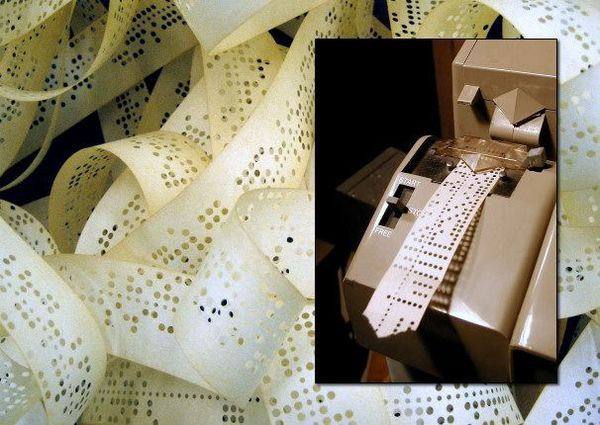
\includegraphics[width=\textwidth]{img/img1.jpg}
	\end{subfigure}
	\begin{subfigure}[b]{0.45\textwidth}
		\centering
		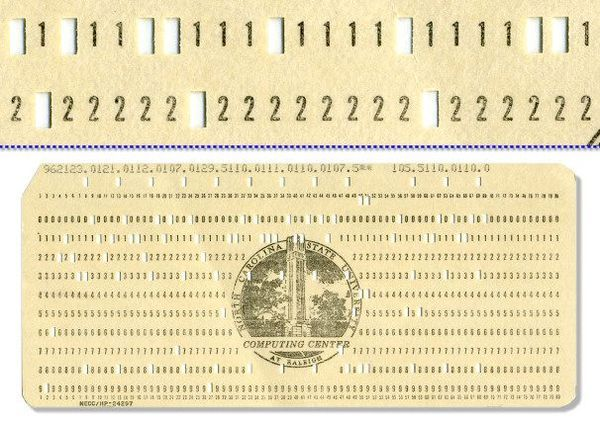
\includegraphics[width=\textwidth]{img/img2.jpg}
	\end{subfigure}
\end{figure}

Вместе с выходом первого американского коммерческого компьютера UNIVAC I (1951) в IT-индустрии началась эра магнитной пленки. Первопроходцем, как водится, снова стала IBM, потом «подтянулись» другие.

В 1963 году IBM представила первый винчестер со съемным диском – IBM 1311. Он представлял собой набор взаимозаменяемых дисков. Каждый набор состоял из шести дисков диаметром 14 дюймов, вмещавших до 2 Мб информации.

\begin{figure}[h]
	\centering
	\begin{subfigure}[b]{0.45\textwidth}
		\centering
		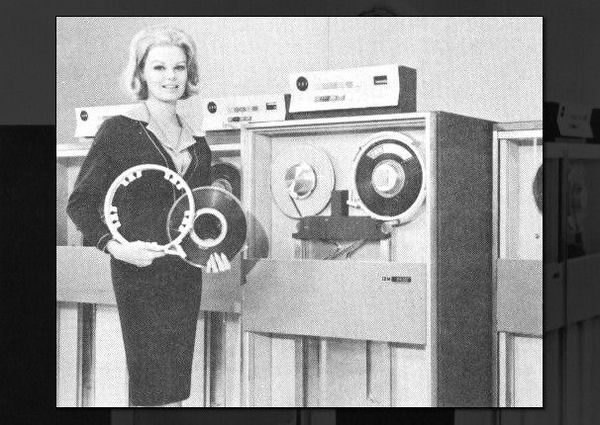
\includegraphics[width=\textwidth]{img/img3.jpg}
	\end{subfigure}
	\begin{subfigure}[b]{0.45\textwidth}
		\centering
		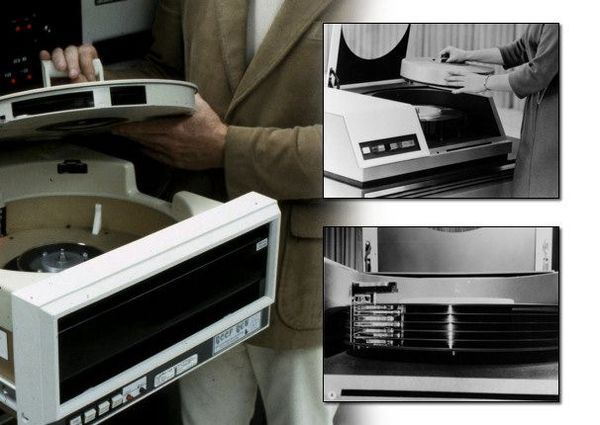
\includegraphics[width=\textwidth]{img/img4.jpg}
	\end{subfigure}
\end{figure}

\end{document}